\section{Angular}\label{sec:angular}

AngularJS\footnote{\url{https://angular.io/}} es un framework para JavaScript utilizado en la creación de aplicaciones web funcionales, también conocidas como aplicaciones de una sola página o en inglés \emph{Single Page Application}. Se trata de un framework de código abierto desarrollado y mantenido por Google. En los últimos años, AngularJS se ha convertido en un framework muy popular dentro de la comunidad de desarrolladores, siendo uno de los más utilizado.

\begin{flushright}
\emph{AngularJS is what HTML would have been, had it been designed for building web-apps. Declarative templates with data-binding, MVW, MVVM, MVC, dependency injection and great testability story all implemented with pure client-side JavaScript!}\\
Web del proyecto AngularJS.
\end{flushright}

AngularJS trata de traer el orden al código de nuestra aplicación. Para ello dispone de las facilidades necesarias a la hora de desarrollar para poder separar la lógica de negocio de la presentación. Se dice que el patrón de arquitectura que sigue es MVW o MV* (Model-View-Whatever!). También se consigue una mejora del rendimiento a la hora de usar AngularJS, entre otras cosas, debido a que no es necesario recorrer el árbol DOM como si que ocurre con otras librerías como \emph{jQuery}.

\begin{figure}
\centering
  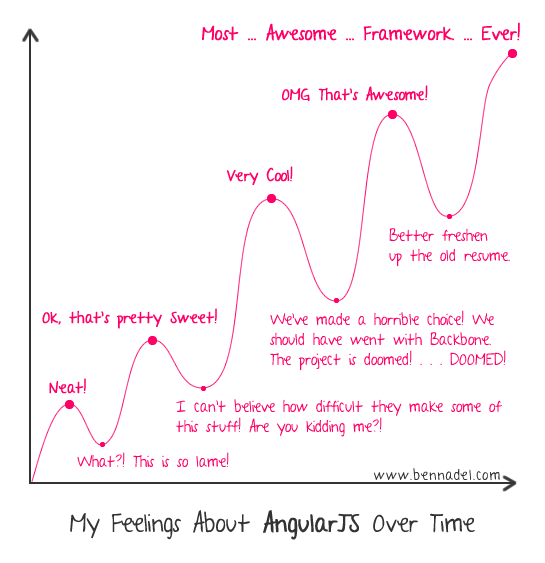
\includegraphics[width=0.8\textwidth]{Figures/ch1/angular/ben_nadel_experience_w_angular}
  \caption{El programador Ben Nadel describió (y de manera muy acertada) su experiencia con Angular en su blog de esta forma. \cite{AngBenNadel}}
\end{figure}

Como ya se vio en la sección \nameref{subsec:frameworkJS}, Angular se ha hecho muy popular siendo hoy en día el framework que goza de más popularidad con diferencia. Esto es importante a la hora de decidir si usarlo o no en nuestro proyecto, ya que nos garantiza el soporte durante los próximos años. Pero hay que tener en cuenta que se trata de un framework complejo, con una curva de aprendizaje que es necesario que tengamos también en cuenta.

Forma parte del stack \gls{MEAN}\footnote{\url{http://mean.io/}} junto con MongoDB, Express y Node.JS. Hablaremos de él mas adelante en el apartado \nameref{subsec:MEAN}.

\subsection{Angular versión 2}

\cite{SharifAng2} Y llego la conferencia europea de AngularJS de 2014 \ldots. En esta conferencia se dio la noticia de que se estaba desarrollando Angular 2.0 y que esta nueva versión sería incompatible con la primera y no habría una hoja de migración desde 1.x a 2.0. En Angular 2.0 se acaba con pilares de la versión tan importantes como es el \emph{\$scope} o los \emph{controladores}, que son sustituidos por los \emph{components}. Estos grandes cambios fueron muy criticados por la comunidad de desarrolladores, los cuales veían como todo lo aprendido iba a dejar der útil. Podemos decir por tanto que más que una segunda versión de AngularJS, se trata de un framework totalmente nuevo.

\tipbox{Angular, AngularJS, Angular2, \ldots ¿Cómo debemos de llamar a este framework?. Pues bien, se ha establecido que:
\begin{enumerate}
  \item Las versiones 1.x serán nombradas como \textbf{AngularJS}.
  \item Las versiones 2.x en adelante tomarán el nombre de \textbf{Angular} a secas.
  \item Se indicará el número de versión si se quiere mencionar a una característica concreta de esta. Por ejemplo, \textbf{Angular 2.4}
  \item La versión \gls{SEMVER} completa si queremos indicar algún bug.
\end{enumerate}}

\tipbox{En el momento de escribir esta memoria, acaba de salir la versión 4 de Angular. Esta nueva versión es compatible hacia atrás con la versión 2. También se anunciado la futurible versión 5.
El motivo de saltar de numeración del 2 al 4 es para unificar la versión de los paquetes del core de Angular ya que estos paquetes se distribuyen por separado y utilizan \gls{SEMVER}. Además, todos estos paquetes se encuentran en la misma versión que Angular excepto uno, \@angular/route, el cual se encuentra en la versión 3.x. Por ello, han decidido saltarse la versión 3 e ir directamente a la 4. }

Aunque Angular es perfectamente compatible con Vanila JavaScript, se recomienda el uso de TypeScript a la hora de programar nuestra aplicación. Gracias a TypeScript el desarrollo será mucho mas sencillo, además, el propio framework está escrito utilizando TypeScript, por lo que la compatibilidad es completa.

\subsubsection{TypeScript}

TypeScript\footnote{\url{https://www.typescriptlang.org/}} es un superconjunto de JavaScript, es decir, se trata de un lenguaje basado en JavaScript, al cuál le añade grandes beneficios. Es por esto que podemos usar código JavaScript en nuestro código TypeScript con la tranquilidad de que va funcionar correctamente. TypeScript implementa todas las funcionalidades que define ECMAScript 6\footnote{\url{http://es6-features.org/}}, añadiendo además algunas propias (algunas de las cuales se plantean introducir en ECMAScript 7).

Para que las aplicaciones escritas usando TypeScript puedan ser usadas en motores de ejecución de JavaScript, por ejemplo en los navegadores, la mayoria de los cuales reconocen ECMAScript 5, el código TypeScript debe ser compilado, lo que hace que sea traducido a JavaScript. Es este código traducido al JavaScript el que es realmente ejecutado por el navegador (o la WebView).

Algunas de las características (parte de las cuales son compartidas por los estándares mencionados antes) que TypeScript añade sobre JavaScript son:

\begin{enumerate}
  \item El uso de clases, haciendo del lenguaje un lenguaje orientado a objetos, lo que es de gran ayuda en proyectos de cierta envergadura.
  \item El tipado de variables y verificación en tiempo de compilación.
  \item Interfaces y herencia.
  \item Uso de anotaciones.
  \item Funciones lambda\footnote{\url{https://basarat.gitbooks.io/typescript/docs/arrow-functions.html}}.
  \item Uso de clases \emph{mixin}\footnote{\url{https://www.typescriptlang.org/docs/handbook/mixins.html}}
  \item \emph{Tuplas} y las \emph{Enumeraciones}.
  \item \ldots
\end{enumerate}

\subsubsection{Aspectos más importantes en Angular}

\cite{Ang2EnrOriol,DiffCompDir} Después del breve apunte sobre TypeScript, sigamos hablando de Angular. Sería necesario bastante más que un capítulo dentro del marco tecnológico de este \gls{PFC} para poder explicar en detalle todas las características que ofrece Angualar2. Por ello, vamos a centrarnos en comentar aquellas más relevantes y así estar algo más preparados a la hora de enfrentarnos a la realización de las prácticas más adelante. Como veremos, Angular se aprovecha de las \emph{clases}, las \emph{anotaciones}, la \emph{herencia}, \ldots que define TypeScript para implementar las funcionalidades que ofrece, por ejemplo, los \emph{componentes} o \emph{directivas} que explicaremos a continuación se implementan como clases con unos metadatos definidos mediante una anotación.

\begin{figure}[h]
\centering
  \includegraphics[width=\textwidth]{Figures/ch1/angular/Angular2_diagram}
  \caption{Esquema de algunos de los elementos que encontramos en una aplicación realizada con Angular y como interactúan entre ellos.}
\end{figure}

\paragraph{Módulos} Angular es modular. Se organiza en módulos los cuales se caracterizan por tener un único objetivo. Estos módulos  suelen exportar ciertos elementos que pueden ser usados por otros módulos. Un ejemplo de módulos serían las librerías que forman Angular y que debemos importar cada vez que queremos usar alguna de sus facilidades.

\notebox{
  Dentro de las librerías de Angular, las más importantes son:
  \begin{enumerate}
    \item @angular/core
    \item @angular/common
    \item @angular/router
    \item @angular/http
  \end{enumerate}
  Veremos el uso de algunas de ellas a lo largo de \nameref{ch:practices}
}

\paragraph{Components}

Una aplicación hecha con \emph{Angular} está formada por \emph{componentes} los cuales cuelgan uno de otros formando una especie de árbol. Existe un  \emph{component} raíz del cual cuelgan el resto de  \emph{componentes}. Esta estructura es similar a la que nos podemos encontrar en un \gls{HTML}, donde todos los elementos se encuentran anidados dentro de otro hasta llegar al elemento \textbf{<body>}.

Un componente está definido por una clase a la que se le añade la anotación \emph{@component}, donde se definen los metadatos del componente, y un \textbf{template} que define la vista (engloba el \gls{HTML} y el \emph{CSS}). Tanto las propiedades como los métodos definidos en un componentes son accesibles desde la vista. Un elemento del \gls{DOM} solo puede estar asociado a un componente.

Los componentes se utilizan para separar la aplicación en pedazos más pequeños.

\paragraph{Data Binding}

En mi opinión, una de las características más potentes de Angular. Gracias al \emph{Data Binding} que ofrece Angular, podemos conectar valores entre la vista y la parte lógica de nuestro componente y convertir acciones que realice el usuario en llamadas a métodos sin tener que escribir toda la lógica que hay detrás de esto.

\paragraph{Directivas}

Una directiva nos permite añadir comportamiento a un elemento \gls{DOM} ya existente. En realidad, los \emph{componentes} son \emph{directiva} con una vista asignada, mientras que una \emph{directiva} puede ser reusada en diferentes elementos del \gls{DOM}, además de poder usar varias sobre un mismo elemento.

Las directivas se definen utilizando la anotación \emph{@directive}, en el que también se definen los metadatos de la directiva.

\paragraph{Servicios}

Los servicios son clases con una funcionalidad específica y que es compartido por los componentes que forman la aplicación. Estos servicios son accesibles desde los diferentes componentes gracias al inyector de dependencias (\emph{Dependency Injection}). Para definir un servicio se utiliza el decorador \emph{@injectable}.

Un uso típico de los servicios es la recuperar datos desde una fuente externa para ser usados en nuestra aplicación.

\paragraph{Dependency Injection}

Este término hace referencia a un mecanismo para proporcionar nuevas instancias de una clase con todas aquellas dependencias que requiere, facilitando así la modularidad. Se utiliza sobretodo para inyectar los servicios a los componentes que los van a usar, y todo esto con solo especificar en el constructor del componente los servicios que espera.

A la hora de crear nuestra aplicación, debemos de indicar los servicios que se van a utilizar a través de un \emph{provider} definido en el módulo lo contiene. Así, el inyector sabe como debe instanciar las dependencias que le "soliciten" los diferentes componentes (u otros servicios).

\subsection{MEAN}\label{subsec:MEAN}

\cite{MEAN} Aunque esta sección está englobada dentro de \nameref{sec:angular}, no nos confundamos, es Angular la que en verdad forma parte del stack \gls{MEAN}\footnote{\url{http://mean.io/}}. Aunque no veremos nada sobre este a lo largo de este \gls{PFC}, y el único componente de los que esta formado y vamos a tratar sea Angular, me ha parecido interesante introducirlo mediante una breve introducción. Pero, ¿a qué nos referimos cuando hablamos del stack \gls{MEAN}?.

Se conoce como stack \gls{MEAN} al conjunto de tecnologías que permiten la creación de aplicaciones distribuidas utilizando únicamente, y en todas sus fases, JavaScript. El nombre se debe a que las cuatro tecnologías principales que lo forman, son \textbf{M}ongoDB, \textbf{E}xpress, \textbf{A}ngular y \textbf{N}odeJS. Esto no quiere decir que no se puedan usar otros elementos como Browser, Selenium, Sass, \ldots para facilitarnos el trabajo.

\begin{figure}[H]
\centering
  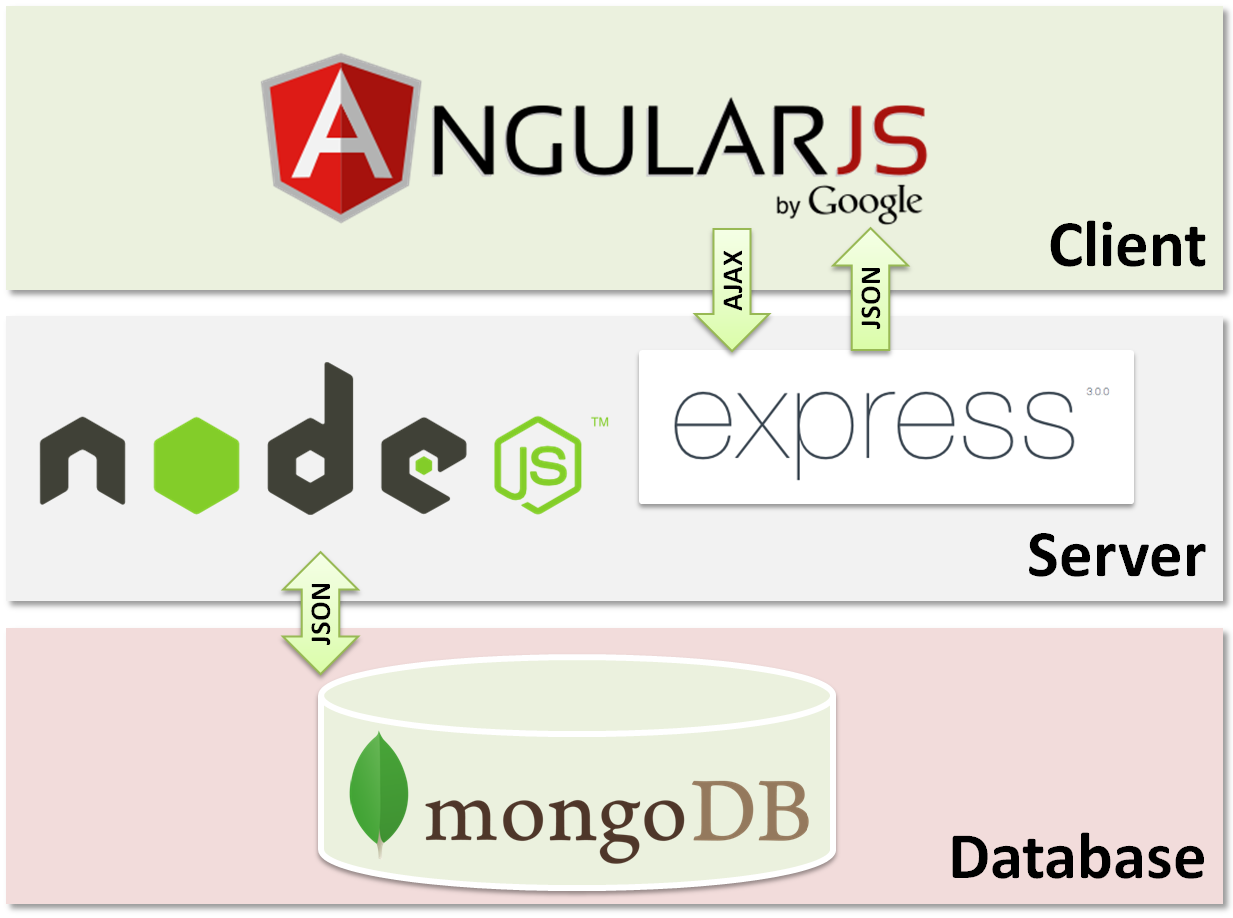
\includegraphics[width=0.8\textwidth]{Figures/ch1/angular/mean}
  \caption{Los cuatro elementos principales del stack en cada una de las fases.}
\end{figure}

\begin{enumerate}
  \item NodeJS: Un entorno de ejecución de JavaScript, basado a su vez en el motor de ejecución V8 desarrollado por Google. Este proyecto ha permitido que JavaScript de el salto del lado del cliente a poder ser usado también en la parte del servidor (aunque en sus inicios ya lo podíamos encontrar, pero no tuvo mucho recorrido). Provee de una arquitectura orientada a eventos (como la de los navegadores) así como una serie de APIs asíncronas que le proporcionan un rendimiento y una escalabilidad muy elevadas.
  \item Express\footnote{\url{http://expressjs.com/}}: Framework utilizado para implementar aplicaciones web sobre NodeJS. Aunque podemos crear nuestro servidor sin necesidad de utilizar ningún tipo de herramienta ajena a NodeJS, ExpressJS nos facilita esta tarea cubriendo las principales necesidades de cualquier servidor web (gestión de peticiones y respuestas, cabeceras, rutas, vistas, \ldots).
  \item MongoDB\footnote{\url{https://www.mongodb.com/}}: En la parte de almacenamiento se encuentra esta \gls{BBDD} \gls{NoSQL} de tipo documental, que almacena la información en un formato similar al \gls{JSON}.
  \item Angular: Utilizado como no podría ser de otra manera para implementar el cliente de la aplicación distribuida.
\end{enumerate}

La razón por la que se ha hecho esta pequeña introducción a \gls{MEAN} es por la importancia que está consiguiendo dentro de la comunidad de desarrolladores. JavaScript se esta posicionando como uno de los lenguajes principales, y herramientas como esta, hacen que su uso no se restrinja a solo el lado del cliente. Además, una aplicación móvil, y de esto si que trata el este \gls{PFC}, suele apoyarse en servidores, por lo que es conveniente saber que alternativas se encuentran disponibles para su implementación, y si es usando un lenguaje (JavaScript) y una tecnología(NodeJS) ya conocida, mejor.

\notebox{
  Por mi experiencia en el desarrollo de aplicaciones distribuidas, recomendaría a un desarrollador sin experiencia en backend empezar con un framework más estructurado y robusto, como puede ser Django (framework para Python), y una vez que se tiene un poco de experiencia, dar el salto (si se quiere) al uso tecnologías relacionadas con NodeJS.
}
